%% ------------------------------------------------------------------------- %%
\chapter{Gradient Boosting Machines}
\label{cap:boosting-intro}

\textit{Gradient Boosting Machines}(GBM) is a machine learning algorithm, based on the idea of additive models from statistics and gradient descent. GBM works by building a forward stagewise additive model by performing gradient descent in function space, as proposed by \cite{gbmdef}. 

Gradient Boosting, especially tree based gradient boosting, has been achieving state-of-the-art results in many datasets (\cite{li2012robust}), especially with tabular data. It is a widely-used machine learning algorithm due to its efficiency, accuracy, and interpretability, according to \cite{ke2017lightgbm}. The \textit{Additive Modeling} technique and the \textit{Gradient Descent} algorithm are key ideas to GBMs, and are briefly introduced below.

%% ------------------------------------------------------------------------- %%
\section{Additive Model}\index{additive!model}\index{regression}
An additive model is a  regression technique suggested by \sloppy{\cite{doi:10.1080/01621459.1981.10477729}}, where the basic idea is to approximate a dataset using a sum of \textbf{smooth functions} of the individual features of the observed data, instead of a complex general regression surface.

Consider a supervised dataset is a set of pairs $\supervised$, where $\xisup$ denotes the $p$-dimensional vector of the $i$-th observation ($p$ is the number of features), and $\yisup$ is the true outcome of the $i$-th observation. An additive model is then described as:

\begin{equation}\label{eq:additive}
\mathbb{E}[\yisup\mid \xisup] = \beta_0 + \sum_{j=1}^pf_j(\xmat_{:, j})
\end{equation}

The $\beta_0$ is the intercept term, and each function $f_j$ is learned from the respective $j$-th feature over all the observations in the dataset. Each of those functions can be estimated using any nonparametric regression technique, such as Gaussian Process Regression, smoothing splines, kernel regression, k-nearest-neighbors, etc.

%% ------------------------------------------------------------------------- %%
\section{Gradient Descent}\index{gradient!descent}\index{descent}
\label{Gradient Descent}

Gradient Descent is an iterative optimization algorithm. As explained by \cite{Ruder2016AnOO}, the basic version of the algorithm is used to \textbf{minimize} an objective function $J(\xmat;\theta)$, parameterized by a model's parameters $\theta \in \mathbb{R}^p$, by using the information gradient vector w.r.t the parameters $\theta$ of the function at a specific point to update the parameters in the opposite direction of this vector. Usually the parameters $\theta$ are updated until a fixed number of iterations is reached, or a convergence is reached. This algorithm uses the learning rate $\eta$ to control how much the coefficients of $\theta$ can change on each iteration.

The basic update rule of the original gradient descent algorithm is defined as

\begin{equation}\label{eq:gradientDescent-update}
    \theta_t = \theta_{t-1} - \eta \cdot \nabla_{\theta_{t-1}} J(\xmat;\theta_{t-1})  
\end{equation}

A gradient descent execution will run the above update $M$ times, and it can be interpreted as generating $M$ vectors $p_m$ of the form $p_m = -\eta\cdot\nabla_{\theta_{m-1}}J(\xmat;\theta_{m-1})$, and  this is a key idea which is important in the mathematical formulation of Gradient Boosting Machines. 
Denoting $p_0 = \theta_0$ (the initial parameters values before optimization), the final optimal parameters $\theta^\star$ can be written as

\begin{equation}\label{eq:gradientDescent-params}
    \theta^\star = \sum_{m=0}^{M}p_m
\end{equation}

%% ------------------------------------------------------------------------- %%
\section{Boosting and \textit{AdaBoost}}\index{boosting}\index{AdaBoost}\index{boost}

The boosting method is a general technique which attempts to "boost" the accuracy of a given machine learning algorithm, answering the following question: "Can a set of weak learners create a single strong learner?". A \textit{weak learner} is a model that performs just slightly better than random guessing. The purpose of boosting is to sequentially apply the \textit{weak learning algorithm} (i.e. an algorithm that produces \textit{weak learners}) to modified versions of the data, producing a sequence of weak classifiers $f_m(x), m = 1, 2, ..., M$, as described by \cite{hastie2009elements}. 

In a superficial level, boosting is similar to another technique called \textit{bagging}, used in the famous \textit{Random Forest} learning algorithm, as both are trying to create a strong learner from an ensemble of weak learners. However, they are fundamentally different: In both bagging and boosting, the variance of the estimates are reduced when the ensemble of learners is created, however the boosting method reduces both the bias and the variance, which makes this technique prone to \textit{overfitting}.

\cite{Schapire:1999:BIB:1624312.1624417} gives a brief overview of the boosting method and its applications, especially the famous \textbf{AdaBoost} algorithm, which was a major breakthrough in Machine Learning research. The original AdaBoost algorithm is designed for classification problems, where the output is either $-1$ or $1$, and the final prediction for a given instance is a weighted sum of each generated weak classifier:

\begin{equation}\label{eq:boosting}
    F_m(x) = sign(\sum_{m=1}^{M}\rho_m\cdot f_m(x))
\end{equation}

The weights $\rho_m$ in equation \ref{eq:boosting} are computed by the boosting algorithm, and the idea is increase the influence of weak learners that are more accurate, while at the same time penalizing the ones that do not predict very well. 

The data modifications done in each step of the boosting procedure is to assign weights $w_i$ for each $\xisup$ in the dataset, based if the instance $\xisup$ was correctly classified or not. The initial weight for all data points is $1/n$, and in the boosting process these weights are adjusted following an exponential function using $\rho_m$ and if the point being updated was correctly classified or not in the last update. One can refer to \cite{hastie2009elements} for a detailed explanation of the AdaBoost algorithm and its formal mathematical description. 

\begin{figure}[!h]
  \centering
  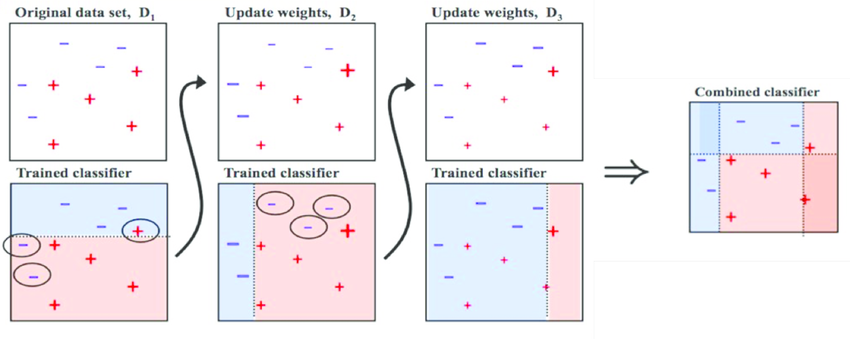
\includegraphics[width=.80\textwidth]{adaboost_classifier.png} 
  \caption{Training of an AdaBoost classifier, image from \cite{adaboost:brendan}}
  \label{fig:humanbeta} 
\end{figure}

%% ------------------------------------------------------------------------- %%
\section{GBMs}\index{boosting}\index{gradient!boosting!machines}\index{boost}

Gradient Boosting Machines were originally introduced by \cite{gbmdef}, in the paper titled "Greedy Function Approximation: A Gradient Boosting Machine". In this work, Friedman makes a connection between stagewise additive expansions (the concept of an additive model) and gradient descent. The GBM algorithm works by optimizing any given differentiable loss function, using gradient descent. However, the optimization is not done in terms of a numeric optimization (i.e. of updating a vector of parameters $\theta$), as described in Section \ref{Gradient Descent}, but by "boosting" functions in the direction of the gradient of the loss function.

Since GBMs deal with finite data, they optimize the functions in terms of the supervised dataset $\supervised$ inputs, not w.r.t all values of $x$, as they're (usually) infinite. The final model of the GBM will be similar to equations \ref{eq:additive} and \ref{eq:boosting}:

\begin{equation}\label{eq:gbm-1}
    F_M(x) = F_0(x) + \sum_{m=1}^M F_m(x)
\end{equation}

The $F_m(x)$ functions are boosted functions built in a stagewise fashion, just like the $\theta_t$ in gradient descent. The base functions are learners, and they can be paremeterized as $\beta_mh(x;a_m)$, where $\beta_m$ is a weight, and $a_m$ the learner parameters. In most implementations the base functions are tree-based learners, but they could be any learner where it is possible to assign weights. Also, given a loss function $L(y_i, F_m(x_i))$, we would like to find all the optimal values of $a_m$ and $\beta_m$ that would minimize the loss function, ie., if we have $M$ functions:

\begin{equation*}
\{\beta_m, a_m\}_1^M = \argmin_{\{\beta_m^\apsimple, a_m^\apsimple\}_1^M} \sum_{i=1}^n L\bigg(\yisup, \sum_{m=1}^M \beta_m^\apsimple h(\xisup;a_m^\apsimple)\bigg)
\end{equation*}

However in most situations the optimization above is infeasible, so the \say{greedy-stagewise} approach is to optimize each pair $(\beta_m, a_m)$ in a stagewise model, that is, for each $m = 1, 2, ..., M$

\begin{equation*}
    (\beta_m, a_m) = \argmin_{\beta, a} \sum_{i=1}^n L(\yisup, F_{m-1}(\xisup) + \beta h(\xisup; a))
\end{equation*}

using a vectorized notation and replacing $\Delta_m(X) =\rho_m h(\xmat; a_m)$,  the update rule of the $F_m$ functions described in \ref{eq:gbm-1} is

\begin{equation}\label{eq:gbm-eta}
    F_m(\xmat) = F_{m-1}(\xmat) + \eta \Delta_m(X)
\end{equation}

The learning rate $\eta$ can also be called the \textit{shrinkage} parameter, as it \say{shrinks} the influence of the new learner. \cite{gbmdef} shows the function $\beta_mh(x; a_m)$ can be interpreted as the best greedy step towards the optimal estimate, which can be represented as $F^\star(x)$(similarly to \ref{eq:gradientDescent-params}). This can be seen as an update of the gradient descent method, as in \ref{eq:gradientDescent-update}. The analogue of $-\nabla_{\theta_{t}}$ in the numerical gradient descent from \ref{Gradient Descent} is the gradient of the loss function $L$ with relation to the last estimate $F_{m-1}(x)$, in the notation used by \cite{gbmdef}:

\begin{equation*}
    -g_m(\xisup) = -\bigg[\frac{\partial L(\yisup, F(\xisup))}{\partial F(\xisup)}\bigg]_{F(x)=F_{m-1}(x)}
\end{equation*}

In literature, this gradient of the loss function $L$ with respect to the last prediction $\ypred_{m-1}$ (i.e. $F_{m-1}(\xmat)$) is sometimes called \textbf{pseudo-residual}, and written as $\residual_{m-1}$. Using a vectorized notation, the \textit{pseudo-residual} can be written as

\begin{equation*}
    \residual_{m-1} = \nabla_{F_{m-1}(\xmat)}L(\ytarget, F_{m-1}(\xmat)) = \nabla_{\ypred_{m-1}}L(\ytarget,\ypred_{m-1})
\end{equation*}


The GBM algorithm fits a learner $h(x; a_m)$ with weight $\beta_m$ using the pseudo-residuals, not the original $\xmat$. The final version of the algorithm is formally defined as

\begin{codebox}
    \Procname{$\proc{gradient\_boost}(\xmat, \ytarget, M, \eta)$}
    \li $F_0(\xmat) = \argmin_{\nu}\sum_{i=1}^n L(\yisup, \nu)$
    \li \For $m \gets 1$ \To $M$
    \li     \Do
                $\residual_{m-1} \gets \nabla_{\ypred_{m-1}}L(\ytarget,\ypred_{m-1})$, where $\ypred_{m-1}=F_{m-1}(\xmat)$
    \li         \Comment Train a base learner minimizing squared error
    \li         $a_m \gets \argmin_{a, \beta}\sum_{i=1}^n\big(\residual_{m-1}^{(i)}-\beta h(\xisup;a)\big)^2$
    \li         $\rho_m \gets \argmin_{\rho}\sum_{i=1}^n L(\yisup, F_{m-1}(\xisup) + \rho h(\xisup;a_m))$
    \li         $\Delta_m(X) =\rho_m h(\xmat; a_m)$
    \li         $F_m(\xmat) \gets F_{m-1}(\xmat) + \eta \Delta_m(X)$
            \End
    \li return $F_M$
    \end{codebox}
    
%% ------------------------------------------------------------------------- %%
\section{\textit{XGBoost} and \textit{LightGBM}}\index{boosting}\index{boost}\index{lightGBM}
\label{lightgbm-explanation}

Even though Gradient Boosting was a known technique used in machine learning, it became widespread with the development of XGBoost, a scalable end-to-end tree boosting system, by \cite{chen2016xgboost}. The main improvements brought by XGBoost was the development of a sparsity-aware algorithm for sparse data and a ``weighted quantile sketch for approximate tree learning''. In general terms, the basic greedy algorithm to find the best split at a given tree node in the boosting process is very computationally demanding, especially when finding splits for continuous variables. In XGBoost an \textit{approximate algorithm} is used for split finding, using quantiles of the feature distribution as split points for continuous variables. 

These improvements and a parallel tree learning architecture are the main reasons of the recent spread of gradient boosting techniques. According to \cite{chen2015xgboost}, ``(XGBoost) has been widely adopted by data scientists and machine learning practitioners. XGBoost has been used as a major system in winner solutions of more than ten machine learning challenges in the past year (2015), most of which are highly competitive. These include highly impactful ones in the field, such as KDDCup. It has also been widely adopted by industry users, including Google, Alibaba and Tencent, and various startup companies.''

\begin{figure}[!h]
    \centering
    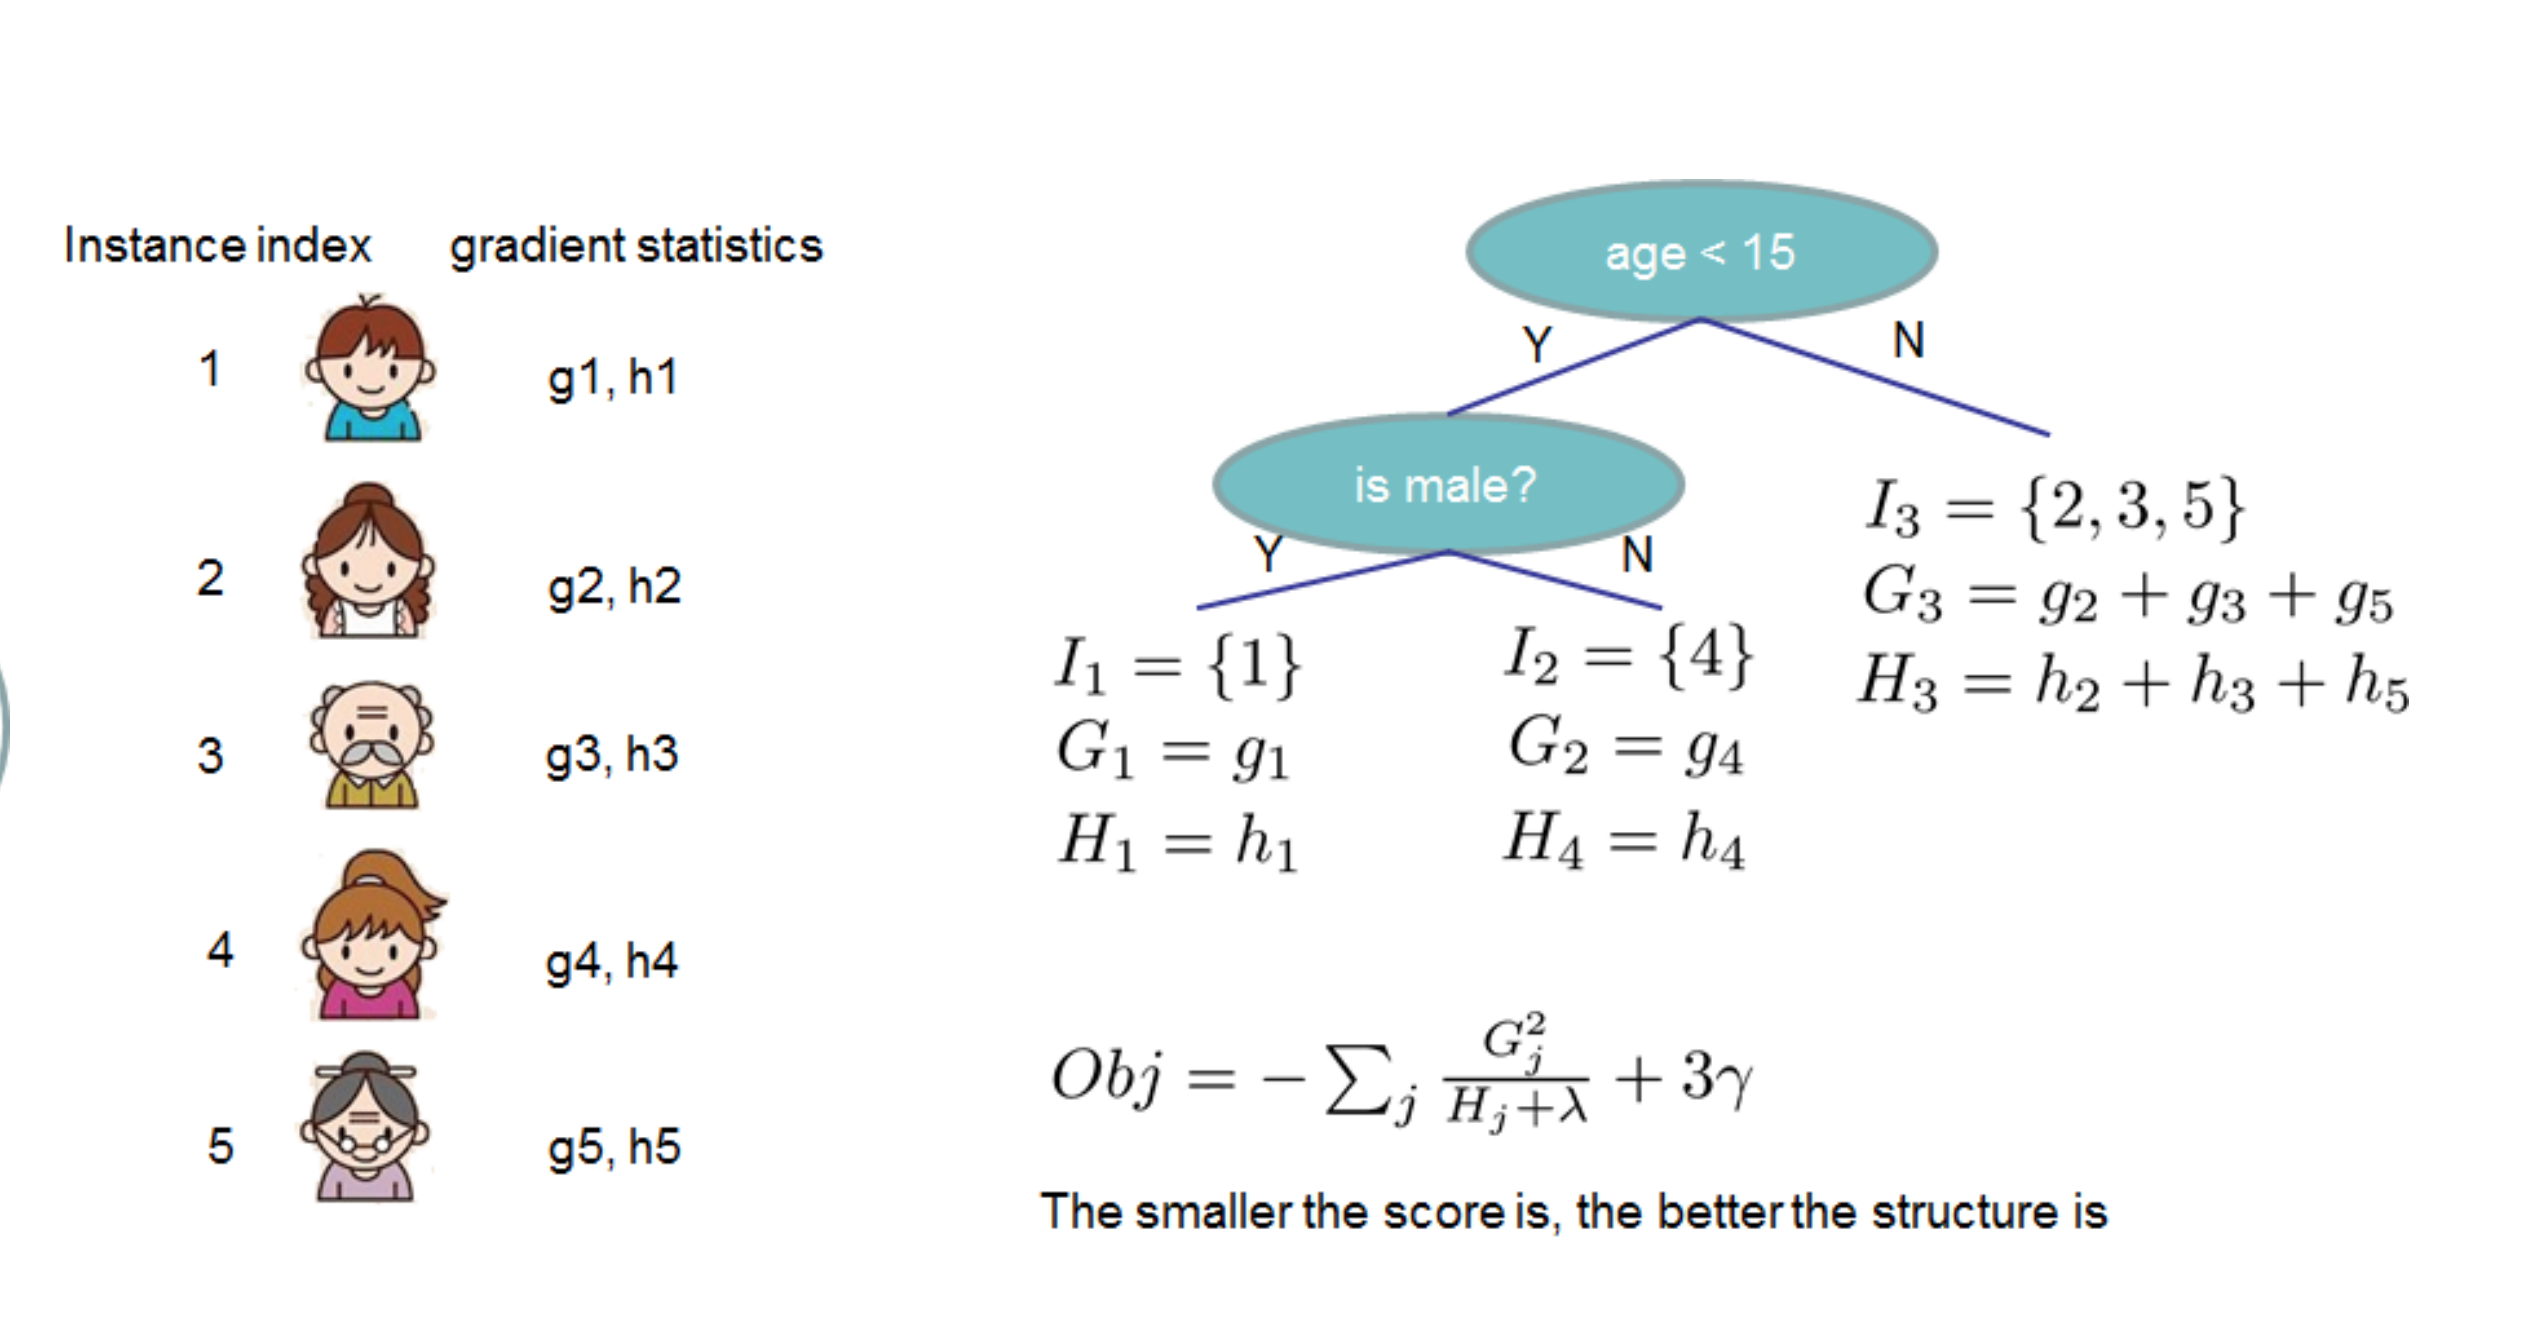
\includegraphics[width=.80\textwidth]{xgboost_tree_structure.png} 
    \caption{Example of structure score calculation for a single tree, from \cite{chen2015xgboost}}
    \label{fig:xgboost-tree} 
  \end{figure}
  

However, the algorithm used in this study is the novel \textbf{LightGBM}, created in 2017 by Microsoft Research in \cite{ke2017lightgbm}. It is important to understand the basic principles and improvements of XGBoost, since its the chosen baseline for performance comparison in XGBoost. There are two main ideas behind LightGBM, both trying to improve the scalability of the gradient boosting process for highly-dimensional data.

First, they propose a new technique for estimation of information gain called \textit{Gradient-based One-Side Sampling} (GOSS). Since one of the most time consuming tasks in the learning process in gradient boosting is to find the split for the trees, usually some sort of sampling is done in this step for efficiency purposes. The researchers noticed that the gradient for each data point in the boosting process has useful information for a smarter data sampling strategy. In the paper \cite{ke2017lightgbm} explains that ``(...) if an instance is associated with a small gradient, the training error for this instance is small and it is already well-trained''. A data sampling strategy is then built based on the rank of the absolute value of the gradient for each instance, sampling instances with higher gradient and subsampling instances with small gradients. The idea is to put more focus on the under-trained instances but keeping the data distribution closer to the original. GOSS has a theoretical proof that its estimation power and generalization performance is close to using the full data, and better than random sampling.

To reduce the number of features, LightGBM develops a technique called \textit{Exclusive Feature Bundling}. It makes use of the high sparsity usually present in high-dimensional data, by designing a `` (...)nearly lossless approach to reduce the number of features''. Since commonly there are many features which are mutually exclusive (never take nonzero values simultaneously), they can be bundled into a single feature. This reduces significantly the algorithmic complexity of the algorithm, since it is basically reducing the number of features. 

Since in this work the impact of \textbf{hyperparameters} from LightGBM is studied, it is important to understand the basics of hyperparameters in these algorithms, covered in the next section.

%% ------------------------------------------------------------------------- %%
\section{Hyperparameters}\index{boosting}\index{gradient!boosting!machines}\index{hyperparameter}
\label{gbm-hyperparams}

One main difference in optimization from other GBM tools is that LightGBM grow trees \textit{leaf-wise} (see Figure \ref{fig:lightgbm-grow}), while most decision tree learning algorithms use a depth-wise approach. This impacts on how each hyperparameter value should be chosen, and which values to optimize. 

\begin{figure}[!h]
    \centering
    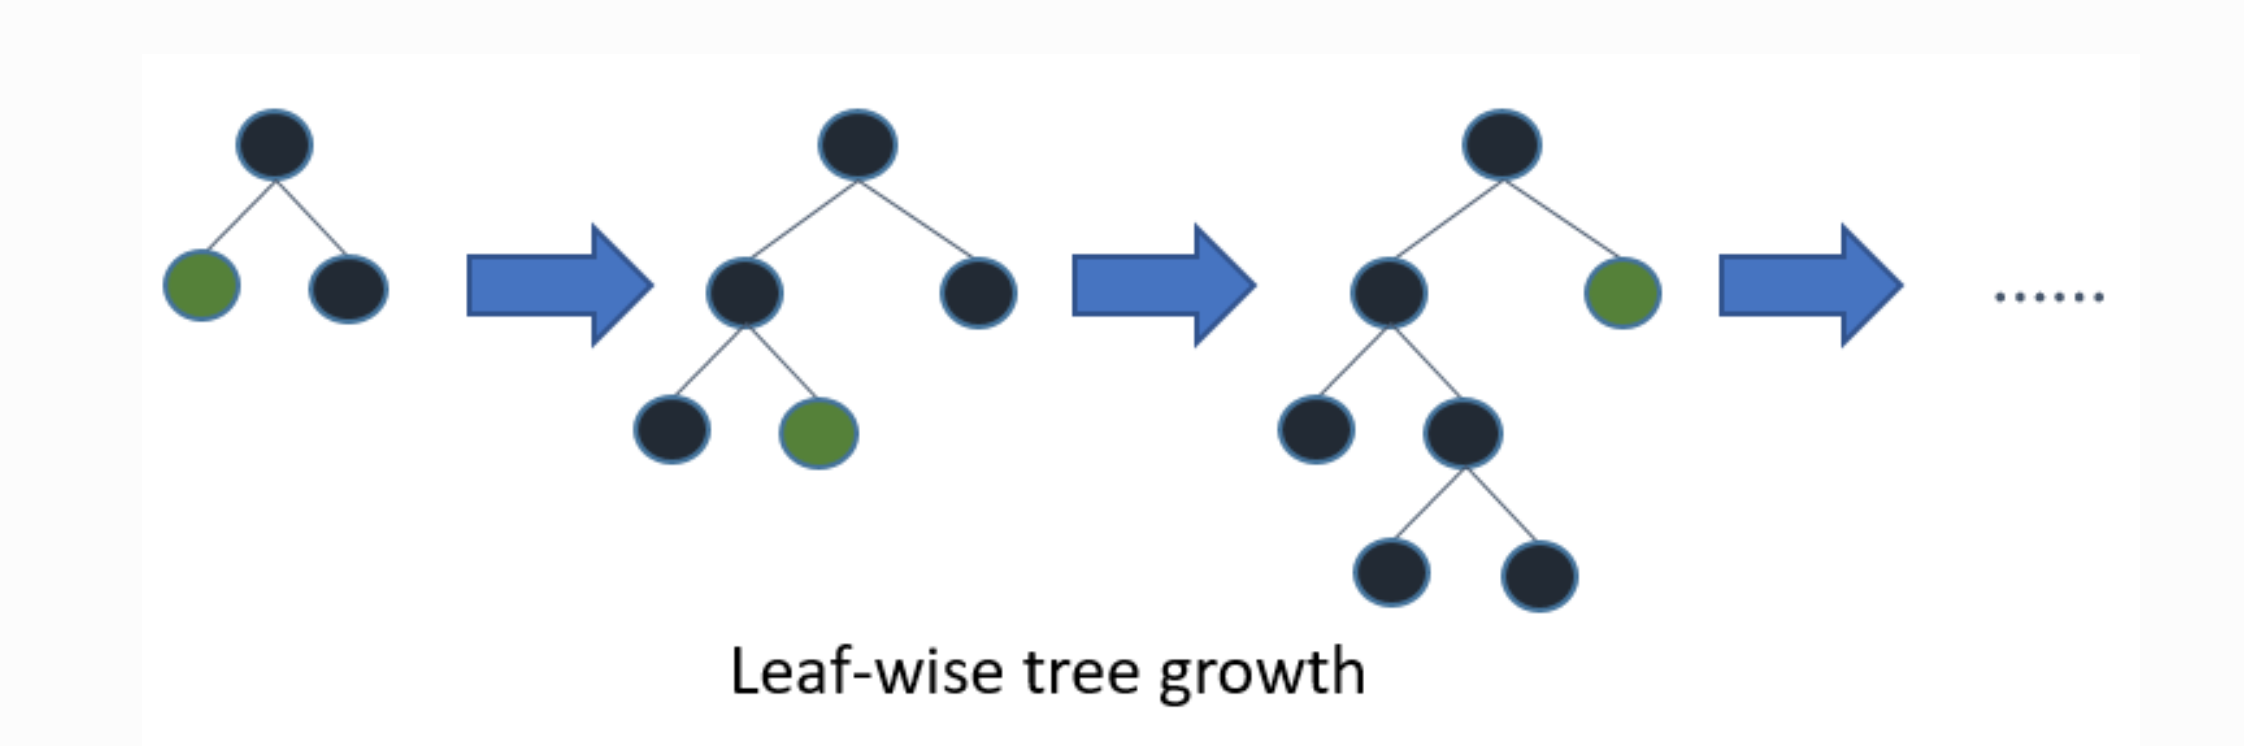
\includegraphics[width=.80\textwidth]{lightgbm_leaf_wise.png} 
    \caption{Leaf-wise tree growth, from LightGBM documentation (\cite{lightgbmparams})}
    \label{fig:lightgbm-grow} 
  \end{figure}

In the documentation from \cite{lightgbmparams}, there are a list of more than 20 hyperparameters one can change and tune when building a gradient boosting model. For tuning the model and controlling complexity, the commonly used hyperparameters to start with are:

\begin{itemize}

    \item \textbf{\code{num\_leaves}}
    
    This hyperparameter control the maximum number of leaves to grow on each boosting iteration, and it is the main way to control the model complexity. By default, LightGBM has no tree maximum depth limit, so this is the main way to apply regularization on the structure of the model. 

    \item \textbf{\code{min\_data\_in\_leaf}}
    
    Controls the minimum number of data points required to grow a new leaf, it is very important since it helps prevent overfitting in leaf-wise trees. From practical experience, this parameter is one of the most sensitive to the number of training samples.

    \item \textbf{\code{max\_depth}}
    
    Controls the depth of each tree explicitly, if needed. In this study, \code{max\_depth} is one of the hyperparameters studied.

    \item \textbf{\code{learning\_rate}}
    
    The learning rate is the parameter $\eta$ from the equation \ref{eq:gbm-eta}, and controls the influence of each new learner. In practice, this is not usually a "tunable" hyperparameter, but rather used in combination with other hyperparameters in the tuning process (e.g. higher learning rate makes the training of the model faster, therefore allowing for faster model tuning). This is one of the hyperparameters analyzed in this study. 

   \item \textbf{\code {n\_estimators}}
   
   The number of estimators or boosting iterations in the gradient boosting process. This is the parameter $M$ in \ref{eq:gbm-1}, and controls how many trees are grown in model training. Usually the larger the number of iterations, the better the model will get, until it starts overfitting in the training data. This is also another hyperparameter analyzed in this study.

\end{itemize}

There are many other parameters in LightGBM, but in practice a model tuning using the models described above usually provide a strong baseline for further tuning.
